\documentclass[11pt]{beamer} 

% Theme (choose one)
\usetheme{McMasterU} % e.g., Madrid, AnnArbor, CambridgeUS, etc.

% Packages
\usepackage[utf8]{inputenc}
\usepackage{amsmath, amssymb}
\usepackage{graphicx}
\usepackage{tikz}
\usetikzlibrary{arrows.meta, positioning, calc}

% Title Information
\title[Topic 5: Arms Race]{Topic 5: Arms Race (Group 10)}
% \subtitle{MATH 3MB3 Final Project}
\author[Jaswal, Khan, Palin, Reeves, and Xu]{Zeyn Jaswal, Azzaam Khan, Timothy Palin, Meredith Reeves, and Tony Xu}
% \institute[McMaster University]{McMaster University}
\date{}

\begin{document}

% Title Frame
\maketitle

% Outline Frame
\section{Overview}
\begin{frame}{Overview}
    
    \textbf{Scenario:} Purple (P) and Green (G) are two countries competing in an arms race.

   \vspace{0.3cm} 

    \textbf{Research Question:} What happens to the long-term spending of each country? 

\vspace{0.3cm}

    \textbf{Key Factors:}
    \begin{itemize}
        \item More inclined to increase defence spending as the other's rises
        \item Less inclined to increase spending as its own spending rises
        \item How does public sentiment affect defence spending?
        \item How does limiting spending affect a country's position?
    \end{itemize}

\vspace{0.3cm}
    \textbf{Motivation:} It helps predict military escalation between countries, which can inform policies to promote peace and prevent conflict.

\end{frame}

% Section
\section{Base Model}
\begin{frame}{Base Model}
    \begin{block}{Model Equations}
        
        The equations for the base model are:

    \begin{equation}
\dfrac{\partial p}{\partial t} = a g(t) - b p(t) + r
\end{equation}

\begin{equation}
\dfrac{\partial g}{\partial t} = c p(t) - d g(t) + s
\end{equation}
    \end{block}
    \begin{itemize}
        \item Feasibility Condition: \((p(t),g(t) \ge 0)\)
        \item \(a,c\): Mutual Fear (\(a,c>0\))
        \item \(b,d\): Defence Spending (\(b,d>0\))
        \item \((r,s)>0\) for trust and \((r,s)<0\) for hostility
    \end{itemize}

% \vspace{0.3cm} 

% \begin{figure}
% \centering

% \begin{tikzpicture}[>=stealth, scale=0.75, every node/.style={transform shape}]

% \node (B) at (-4,0) {B};
% \node[draw, circle, minimum size=1cm] (P) at (0,0) {P};
% \node[draw, circle, minimum size=1cm] (G) at (5,0) {G};
% \node (D) at (9,0) {D};

% \draw[->] (P) -- node[above] {Arms Spending} (B);
% \draw[->] (G) -- node[above] {Arms Spending} (D);

% \draw[->] (P) .. controls (2.5,1) .. node[midway, above] {$PC$ (Fear Factor)} (G);
% \draw[->] (G) .. controls (2.5,-1) .. node[midway, below] {$AG$ (Fear Factor)} (P);

% \end{tikzpicture}

% \caption{Base Model}
% \label{fig:base-model}
% \end{figure}
    
    \end{frame}

% Section
% \iffalse %tentatively removed
% \section{Stability Analysis}
% \begin{frame}{Stability Analysis}    
%     \begin{block}{In the long run, we expect either:}
%      \begin{enumerate}
%         \item Military spending of both countries to stabilize around 
%         \[(p^*(t),g^*(t)) = \bigg(\frac{as+rd}{bd-ac},\frac{cr+sb}{bd-ac}\bigg)\]
%         \begin{enumerate}
%         \item Entails mutual disarmament given the right \(r,s\) values
%         \end{enumerate}
%         \item Military spending of both countries to prepetually increase
%     \end{enumerate}
%     \end{block}
%     \textbf{Case 1 happens if:} $bd>ac$ (i.e. the product of expenditure factors are greater than 
%     mutual fear factors)
% \end{frame}
% \fi

\begin{frame}{Long Term Behavior}
    When both countries are neutral ($r=s=0$), we have:
    \begin{columns}[t]
        \column{0.33\textwidth}
        \begin{center}
        \textbf{$bd>ac$}
        \end{center}
        \column{0.33\textwidth}
        \begin{center}
        \textbf{$bd=ac$}
        \end{center}
        \column{0.33\textwidth}
        \begin{center}
         \textbf{$bd<ac$}
        \end{center}
    \end{columns}
    \begin{columns}[t]
        \column{0.33\textwidth}
        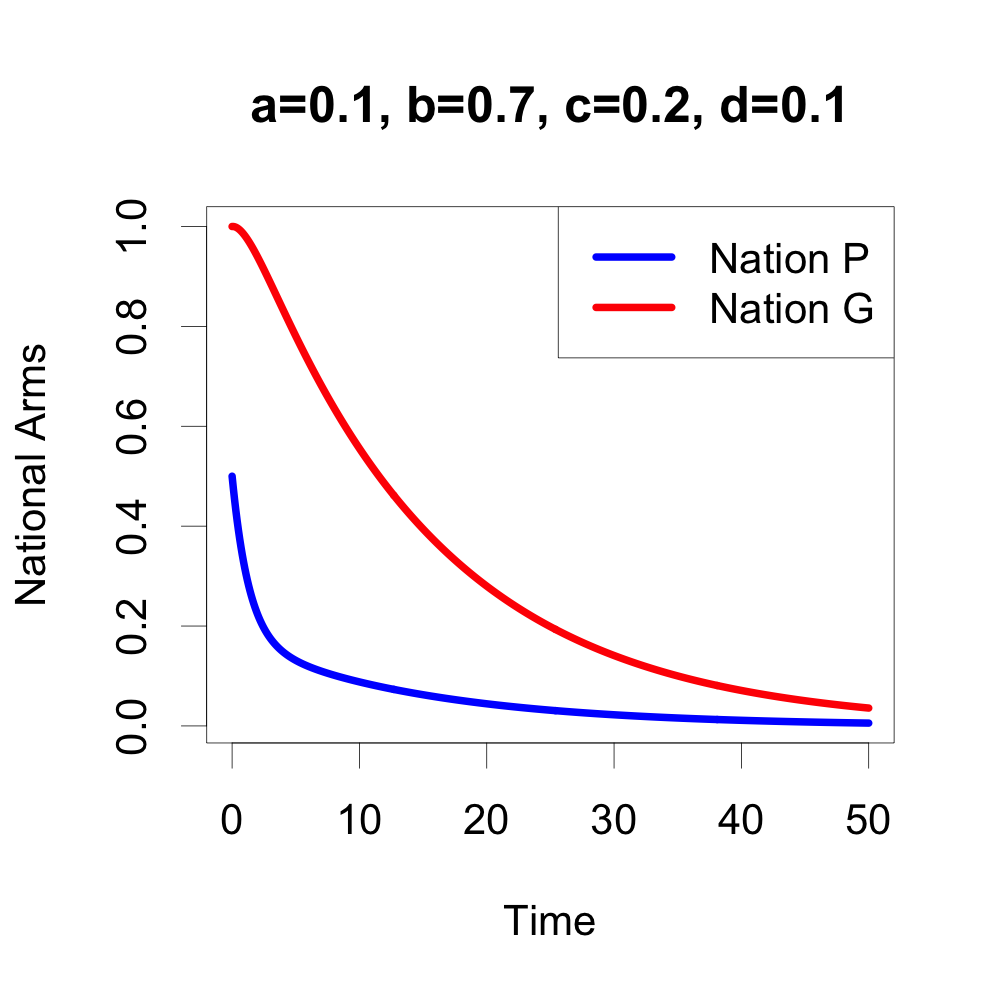
\includegraphics[width=1\textwidth]{bdgeac.png}
        \column{0.33\textwidth}
        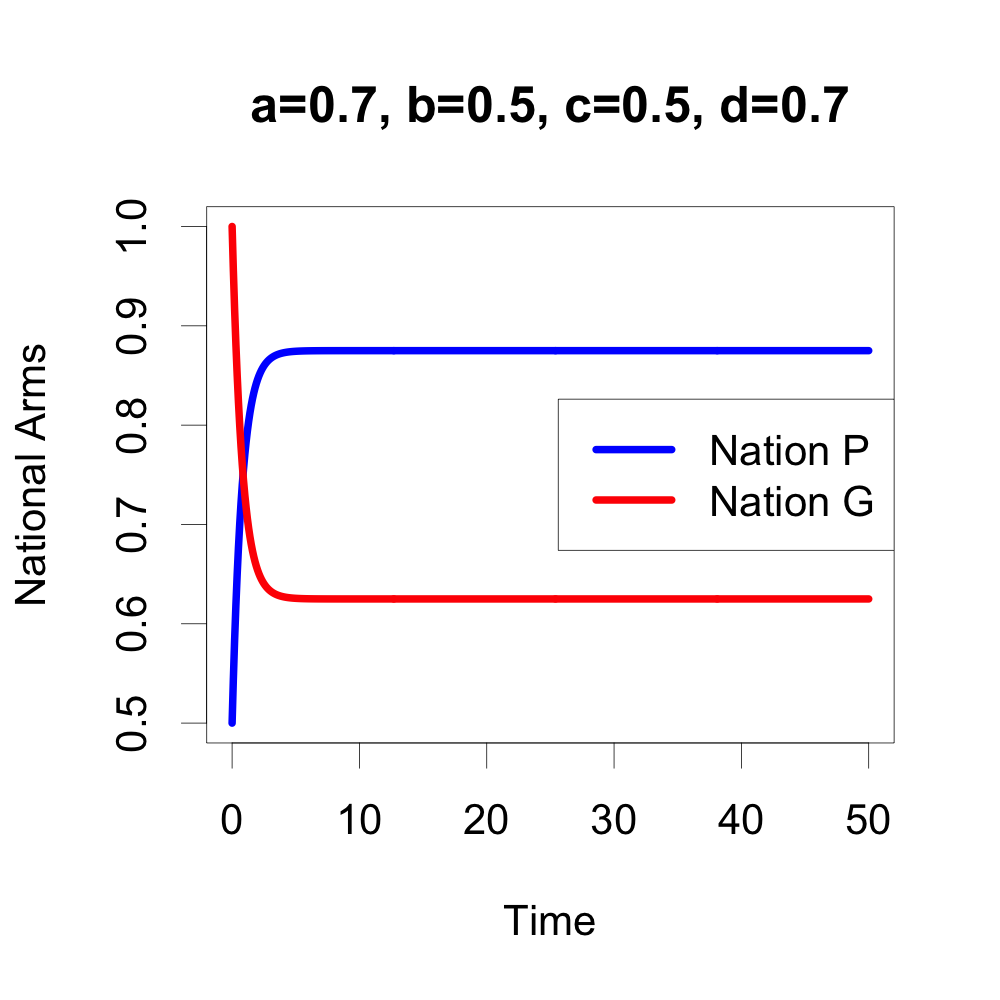
\includegraphics[width=1\textwidth]{bdeqac.png}
        \column{0.33\textwidth}
        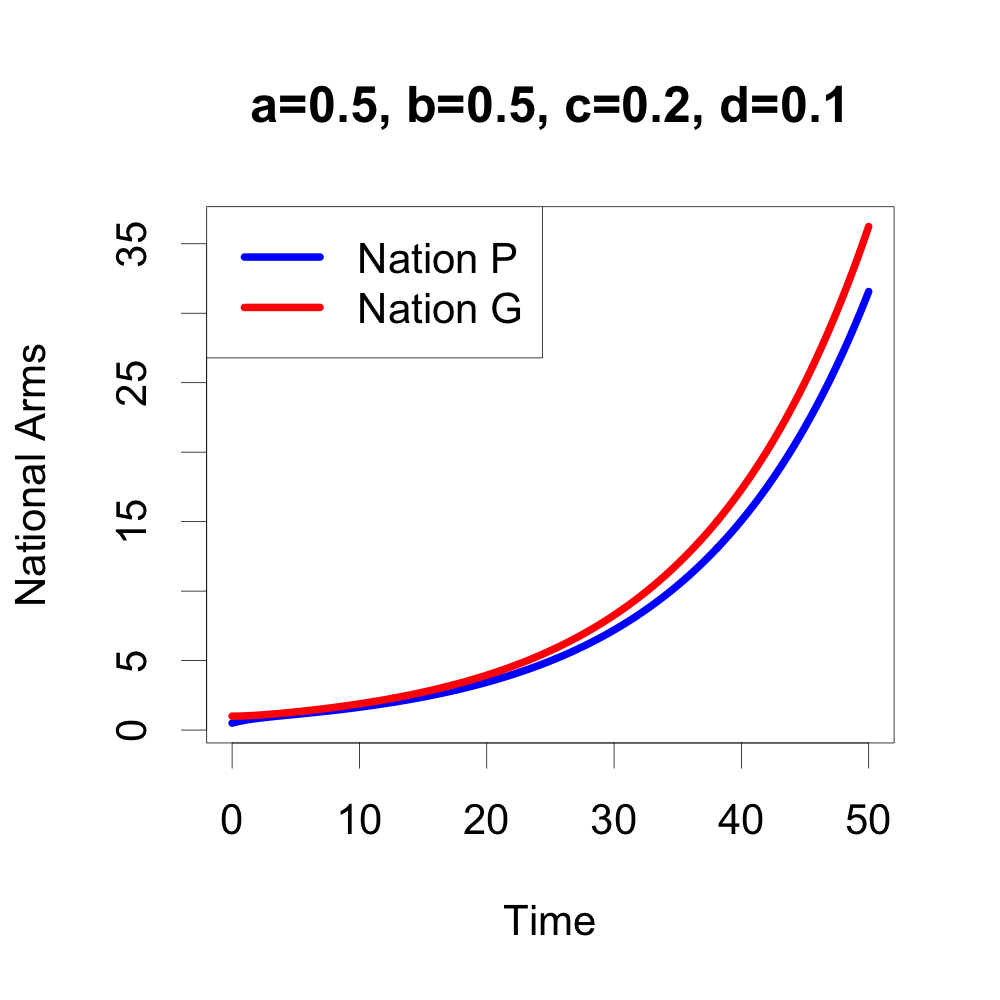
\includegraphics[width=1\textwidth]{bdleac.png}
    \end{columns}
    
\vspace{0.3cm}

    \begin{columns}[t]
    \column{0.33\textwidth}
        \centering
        Complete mutual disarmament \\
        %\((p^\infty,g^\infty)=(0,0)\)
    \column{0.33\textwidth}
        \centering
        Stabilized spending \\
        %\((p^\infty,g^\infty)=(\frac{cp_0+bg_0}{a+c},\frac{dp_0+ag_0}{a+c})\)
    \column{0.33\textwidth}
        \centering
        Perpetual arms race \\
        %\((p^\infty,g^\infty)=(\infty,\infty)\)
    \end{columns}
\end{frame}

% Section 
%\section{Public Sentiment (Trust and Hostility)}
%\begin{frame}{Public Sentiment (Trust and Hostility)}
%    % If P and G have underlying goodwill/grievances that influence their spending \\
%    % The model equations are therefore:
%    \begin{block}{Model Equations}
%        
%        The equations after including public sentiment are:
%    \begin{align*}
%        \dfrac{\partial p}{\partial t} &= a g(t) - b p(t) + r\\
%        \dfrac{\partial g}{\partial t} &= c p(t) - d g(t) + s
%    \end{align*}
%    \end{block}
%    \begin{itemize}
%        \item \((r,s)>0\) for trust and \((r,s)<0\) for hostility
%        % \item Provide further elaborating points
%    \end{itemize}
  
% \vspace{0.3cm}
    
% \begin{figure}
% \centering   

% \begin{tikzpicture}[>=stealth, scale=0.75, every node/.style={transform shape}]

% \node (B) at (-4,-1.5) {B};
% \node (R) at (-4,1.5) {R};
% \node[draw, circle, minimum size=1cm] (P) at (0,0) {P};
% \node[draw, circle, minimum size=1cm] (G) at (5,0) {G};
% \node (S) at (9,1.5) {S};
% \node (D) at (9,-1.5) {D};

% \draw[<-] (P) -- node[midway, above, sloped] {Public Sentiment} (R);
% \draw[<-] (G) -- node[midway , above, sloped] {Public Sentiment} (S);
% \draw[->] (P) -- node[midway, above, sloped] {Arms Spending} (B);
% \draw[->] (G) -- node[midway, above, sloped] {Arms Spending} (D);

% \draw[->] (P) .. controls (2.5,1) .. node[midway, above] {$PC$ (Fear Factor)} (G);
% \draw[->] (G) .. controls (2.5,-1) .. node[midway, below] {$AG$ (Fear Factor)} (P);

% \end{tikzpicture}

% \caption{Base Model Including Public Sentiment}
% \label{fig:publicsentiment-model}
% \end{figure}

%\end{frame}

% \begin{frame}{Long Term Behavior (Public Sentiment)}
% \vspace={1.0cm}
%     \begin{columns}
%         \column{0.5\textwidth}
%         \begin{center}
%         \textbf{$bd>ac$ or $bd=ac, r<0, s<0$}
%         \end{center}
%         \column{0.5\textwidth}
%         \begin{center}
%          \textbf{$bd<ac$ or $bd=ac,r \geq,s>0$}
%         \end{center}
%     \end{columns}
%     \begin{columns}
%         \column{0.5\textwidth}
%         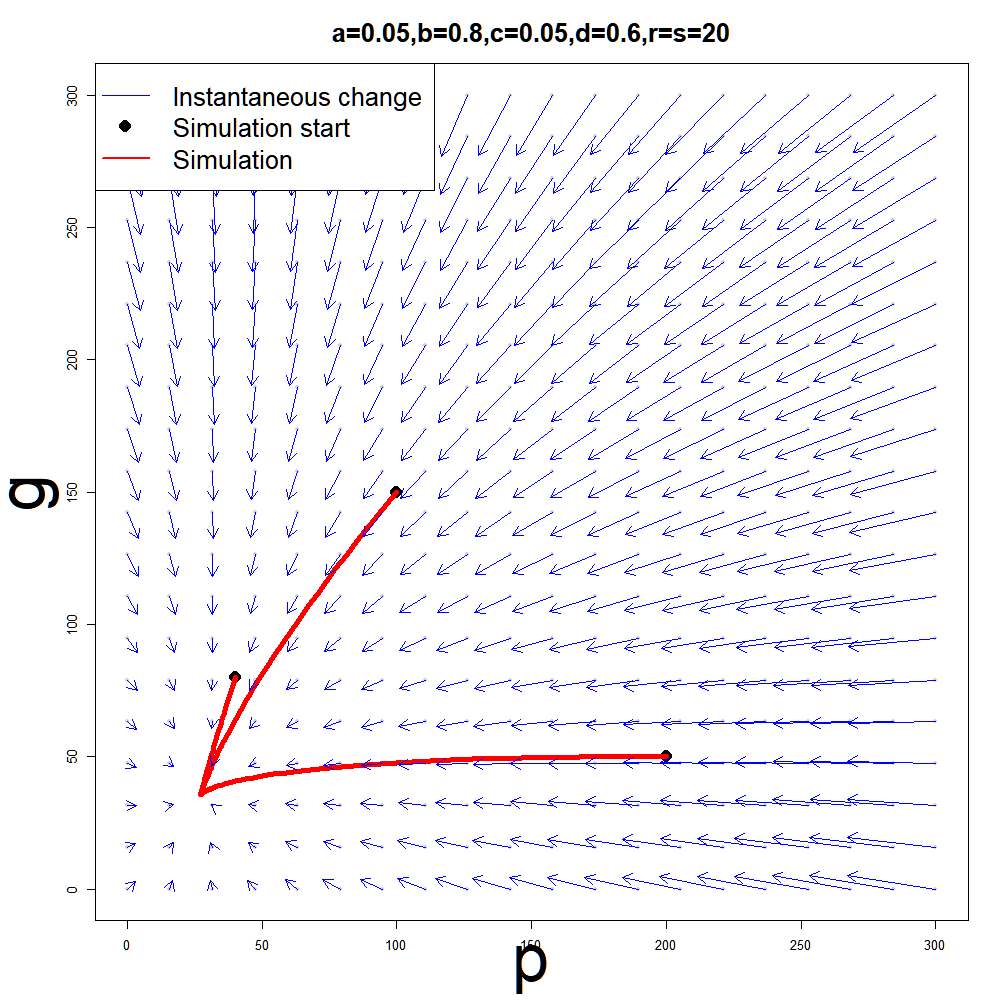
\includegraphics[width=1\textwidth]{S1_bd_gt_ac.png}
%         \column{0.5\textwidth}
%         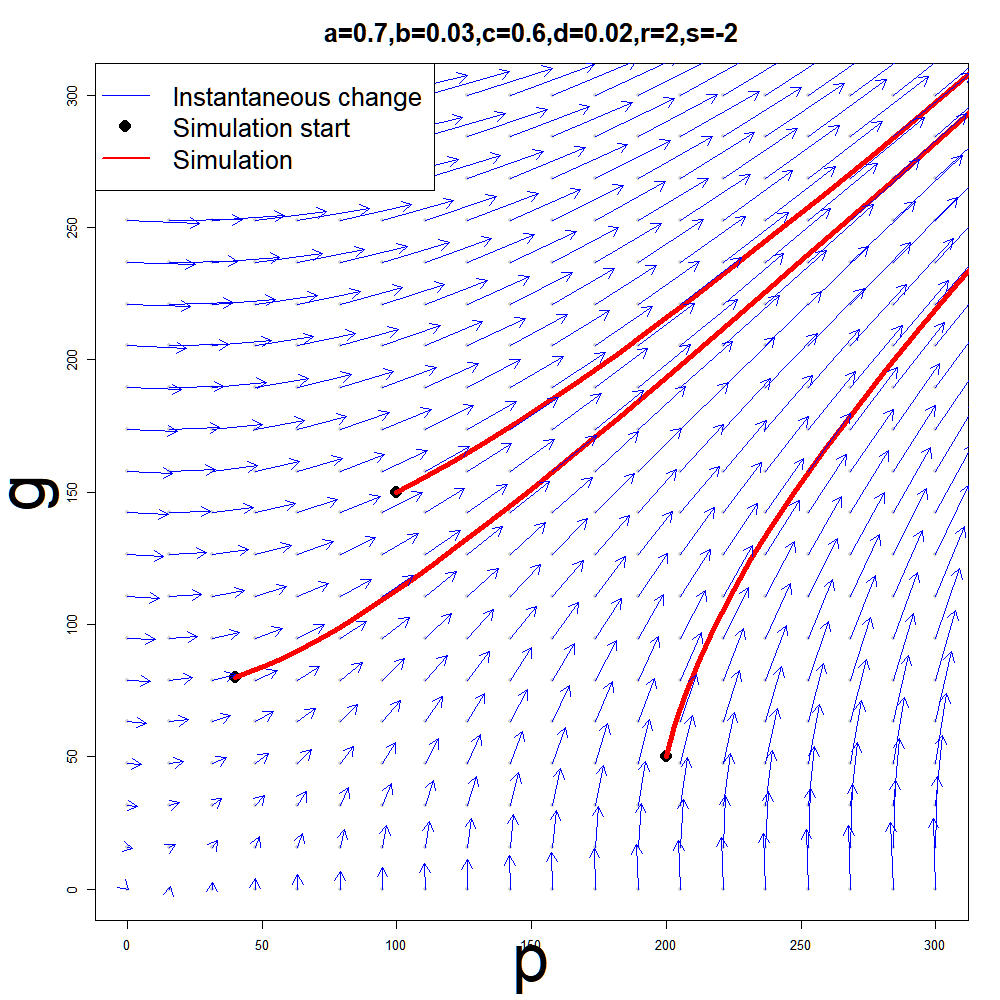
\includegraphics[width=1\textwidth]{S2_bd_lt_ac.png}
%     \end{columns}
    
% \vspace{0.3cm}

%     \begin{columns}
%     \column{0.5\textwidth}
%         \centering
%         Complete mutual disarmament \\
%         %\((p^\infty,g^\infty)=(0,0)\)
%     \column{0.5\textwidth}
%         \centering
%         Perpetual arms race \\
%         %\((p^\infty,g^\infty)=(\infty,\infty)\)
%     \end{columns}
% \end{frame}

%\begin{frame}{Long Term Behavior (Public Sentiment)}
%
%\vspace{0.1cm}
%
%    \begin{columns}
%        \column{0.5\textwidth}
%        \centering
%        \textbf{\small $bd>ac$ or $bd=ac, r<0, s<0$}\\
%        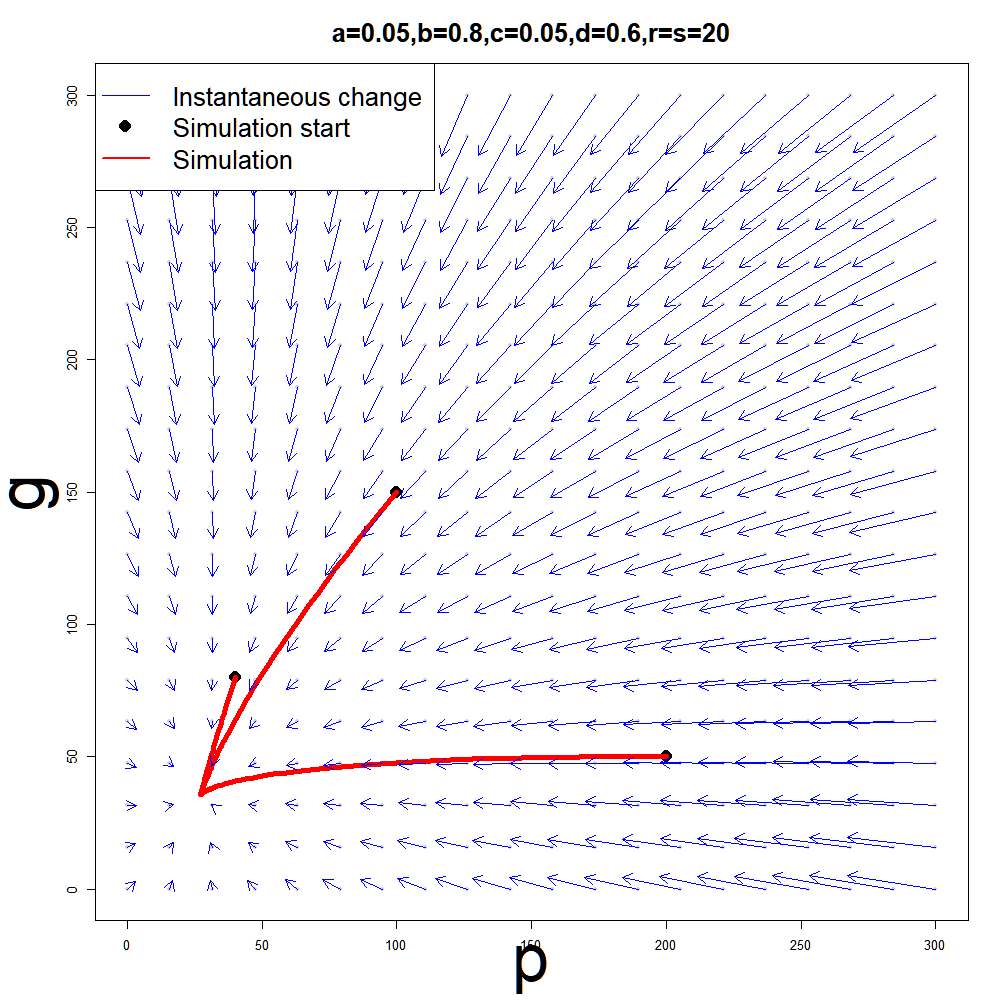
\includegraphics[width=0.5\textwidth]{S1_bd_gt_ac.png}\\
%        \tiny Complete mutual disarmament
%        \column{0.5\textwidth}
%        \centering
%        \textbf{\small $bd<ac$ or $bd=ac,r \geq,s>0$}\\
%        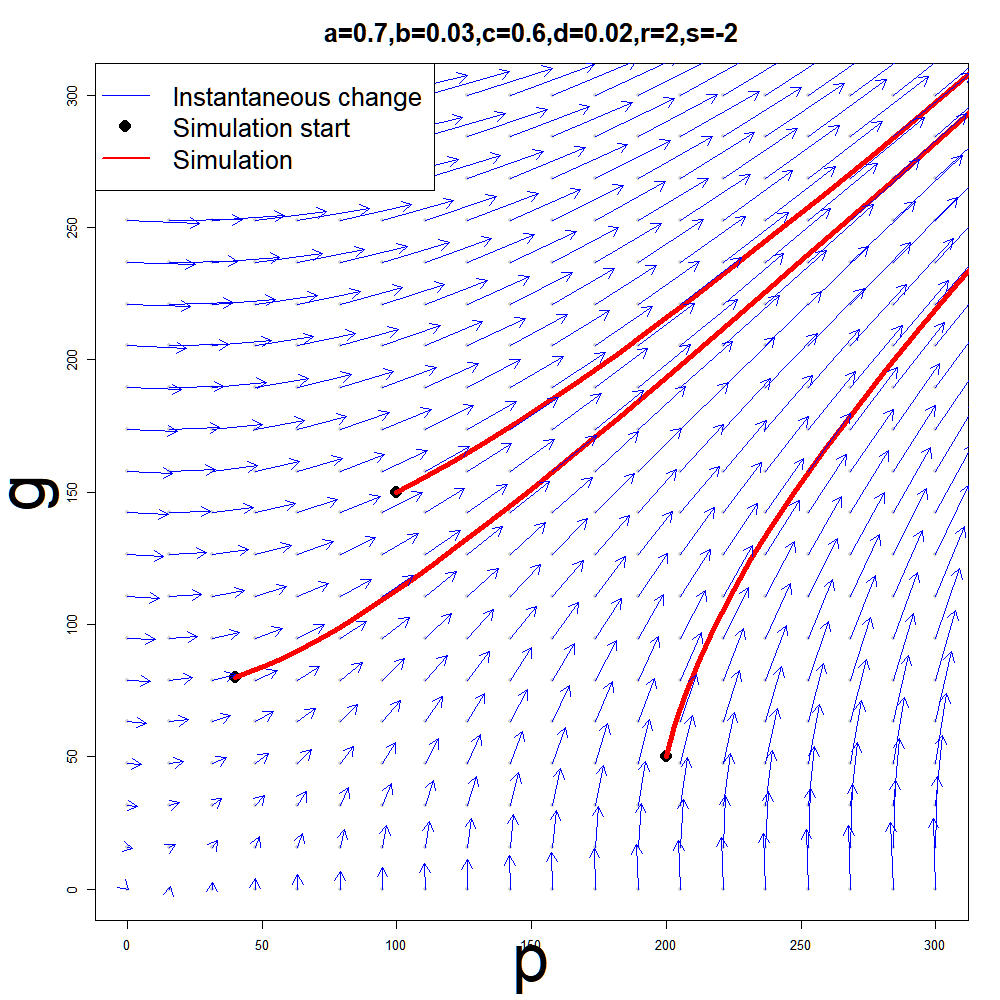
\includegraphics[width=0.5\textwidth]{S2_bd_lt_ac.png}\\
%        \tiny Perpetual arms race
%    \end{columns}
%
%\vspace{0.1cm}
%
%    \begin{columns}
%        \column{0.5\textwidth}
%        \centering
%        \textbf{\small $bd=ac, r<0, s>0$}\\
%        
\includegraphics[width=0.5\textwidth]{S4_bd_eq_ac.png}\\
%        \tiny One nation grows, other nation shrinks
%        \column{0.5\textwidth}
%        \centering
%        \textbf{\small $bd=ac, r=0, s=0$}\\
%        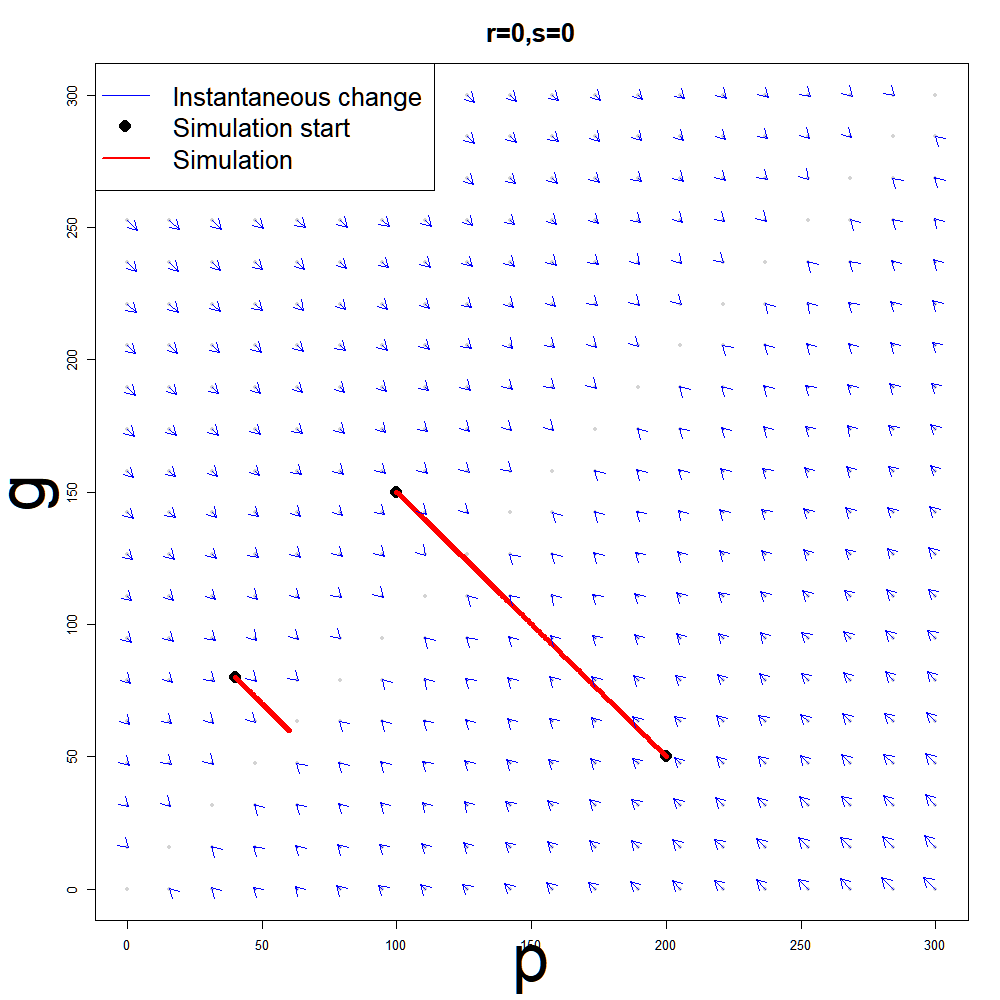
\includegraphics[width=0.5\textwidth]{S7_bd_eq_ac.png}\\
%        \tiny Nations never reach equilbrium
%    \end{columns}
%
%\end{frame}


\begin{frame}{Long Term Behavior}

\vspace{0.1cm}

    \begin{columns}[t]
        \column{0.333\textwidth}
        \centering
        \textbf{\small $bd<ac$, $r<0$, $s<0$}\\
        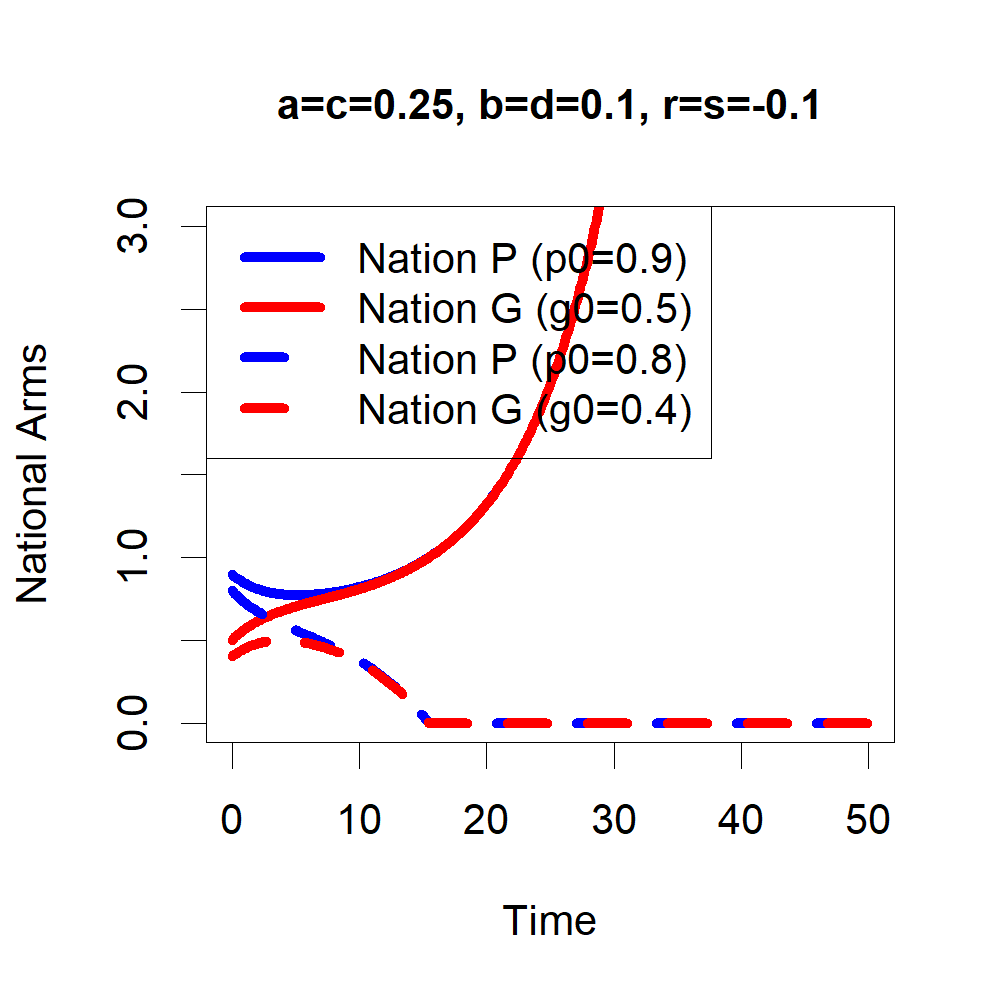
\includegraphics[width=1\textwidth]{rs_p1.png}\\
        Arms equilibrium determined by initial spending
        
        \column{0.333\textwidth}
        \centering
        \textbf{\small $bd=ac$ $r<0$, $s>0$}\\
        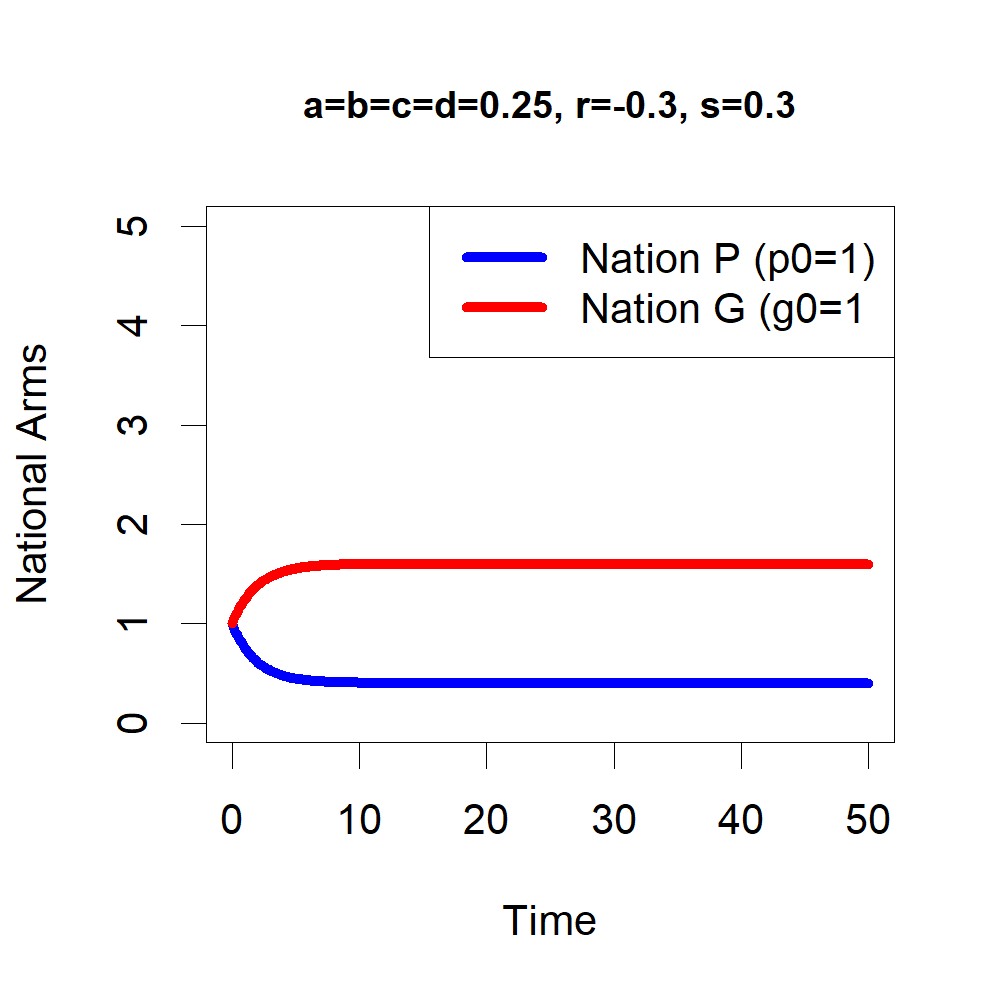
\includegraphics[width=1\textwidth]{rs_p2.png}\\
        Stable arms spending

        \column{0.333\textwidth}
        \centering
        \textbf{\small $bd>ac$, $r>0$, $s>0$}
        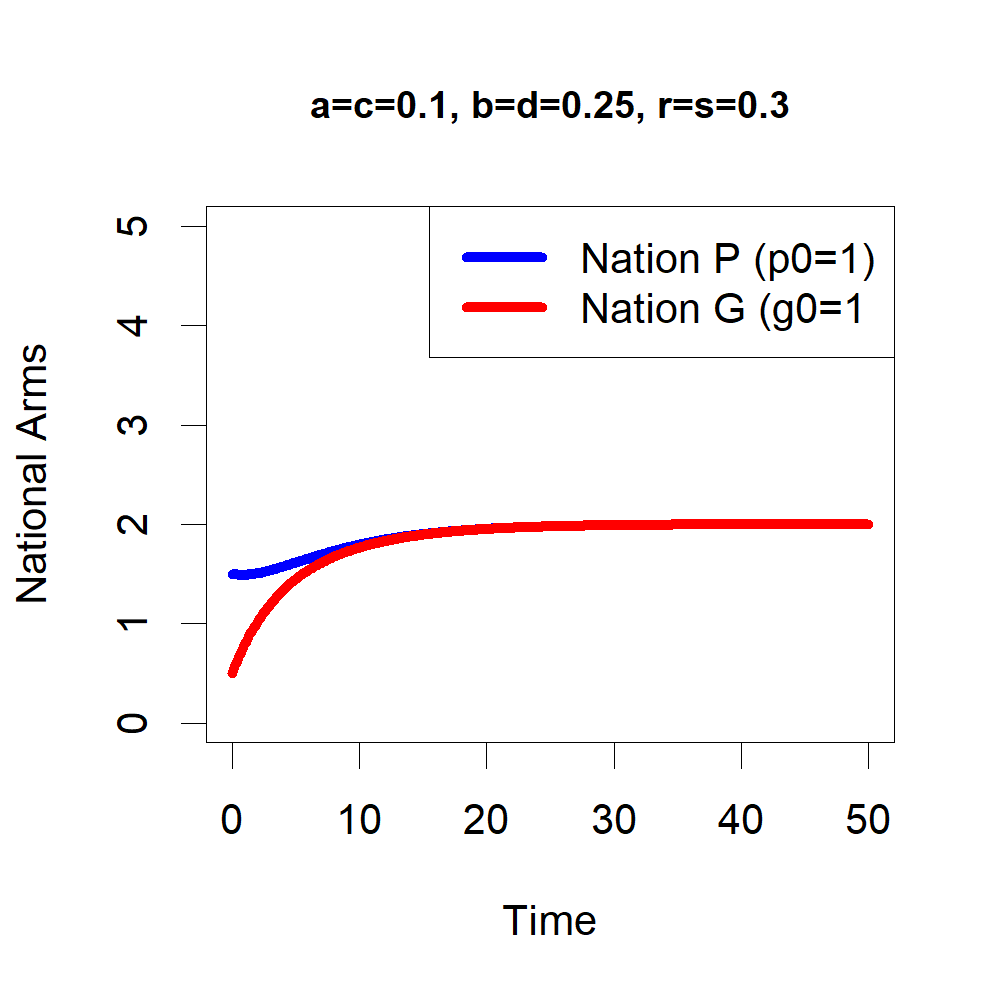
\includegraphics[width=1\textwidth]{rs_p3.png}\\
        Stable arms spending
        
    \end{columns}

\end{frame}

% Section 
\section{Mutual Logistic Fear}
\begin{frame}{Mutual Logistic Fear}
    \textbf{Limitation of the Current Model}: Each country has a limited amount of resources at a given time.
\vspace{0.3cm}

    \textbf{Solution}: Introduce self limiting logistic growth.
     
\vspace{0.3cm}
    \begin{block}{Model Equations}
        The equations after adding logistic growth are:
   \begin{equation}
        \dfrac{\partial p}{\partial t} = a \left (1-\frac{p(t)}{K_p} \right) g(t) - b p(t) + r
    \end{equation}

   \begin{equation}
        \dfrac{\partial g}{\partial t} = c \left (1-\frac{g(t)}{K_g} \right)  p(t) - d g(t) + s
    \end{equation}
    \end{block}

% \vspace{0.3cm}

% \begin{figure}
% \centering   

% \begin{tikzpicture}[>=stealth, scale=0.55, every node/.style={transform shape}]

% \node (B) at (-4,-1.5) {B};
% \node (R) at (-4,1.5) {R};
% \node[draw, circle, minimum size=1cm] (P) at (0,0) {P};
% \node[draw, circle, minimum size=1cm] (G) at (5,0) {G};
% \node (S) at (9,1.5) {S};
% \node (D) at (9,-1.5) {D};

% \draw[<-] (P) -- node[midway, above, sloped] {Public Sentiment} (R);
% \draw[<-] (G) -- node[midway , above, sloped] {Public Sentiment} (S);
% \draw[->] (P) -- node[midway, above, sloped] {Arms Spending} (B);
% \draw[->] (G) -- node[midway, above, sloped] {Arms Spending} (D);

% \draw[->] (P) .. controls (2.5,1) .. node[midway, above] {$PC$ (Fear Factor)} (G);
% \draw[->] (G) .. controls (2.5,-1) .. node[midway, below] {$AG$ (Fear Factor)} (P);
% \draw[->] (P) to[out=130,in=60,loop, looseness=7] node[above] {Mutual Fear} (P);
% \draw[->] (G) to[out=130,in=60,loop, looseness=7] node[above] {Mutual Fear} (G);

% \end{tikzpicture}

% \caption{Base Model Including Public Sentiment and Mutual Fear}
% \label{fig:mutualfear-model}
% \end{figure}

\end{frame}

\begin{frame}{Long Term Behavior}

\begin{columns}[T]
    \column{0.33\textwidth}
    \centering
    \textbf{$bd > ac$}\\
    
\includegraphics[width=\linewidth]{logistic_case1.png}\\
    \small Complete mutual disarmament

    \column{0.33\textwidth}
    \centering
    \textbf{$bd = ac$}\\
    
\includegraphics[width=\linewidth]{logistic_case2.png}\\
    \small Stabilized spending

    \column{0.33\textwidth}
    \centering
    \textbf{$bd < ac$}\\
    
\includegraphics[width=\linewidth]{logistic_case3.png}\\
    \small Perpetual arms race
\end{columns}

\vspace{0.4cm}

% \begin{itemize}
%     \item Stability depends on relative strength of fear ($b,d$) vs restraint ($a,c$)
%     \item Convergence:
%     \begin{itemize}
%         \item $bd > ac$ $\rightarrow$ decay to zero (disarmament)
%         \item $bd = ac$ $\rightarrow$ steady-state equilibrium
%         \item $bd < ac$ $\rightarrow$ unbounded growth (arms race)
%     \end{itemize}
% \end{itemize}

\end{frame}

% \begin{frame}{Long Term Behavior (Mutual Logistic Fear)}

% \begin{columns}[T]
%     \column{0.33\textwidth}
%     \centering
%     \textbf{$bd > ac$}\\
%     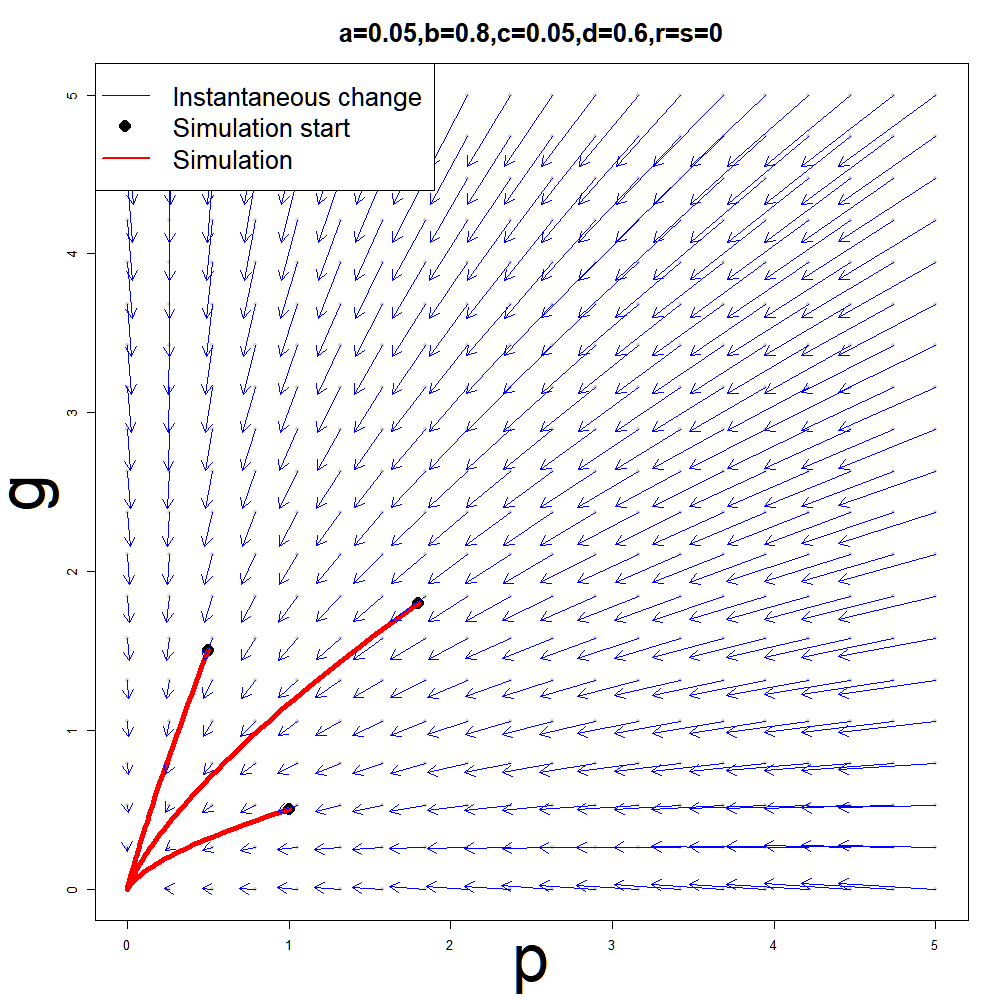
\includegraphics[width=\linewidth]{S1_only_origin.png}\\
%     \small Complete mutual disarmament

%     \column{0.33\textwidth}
%     \centering
%     \textbf{$bd < ac$}\\
%     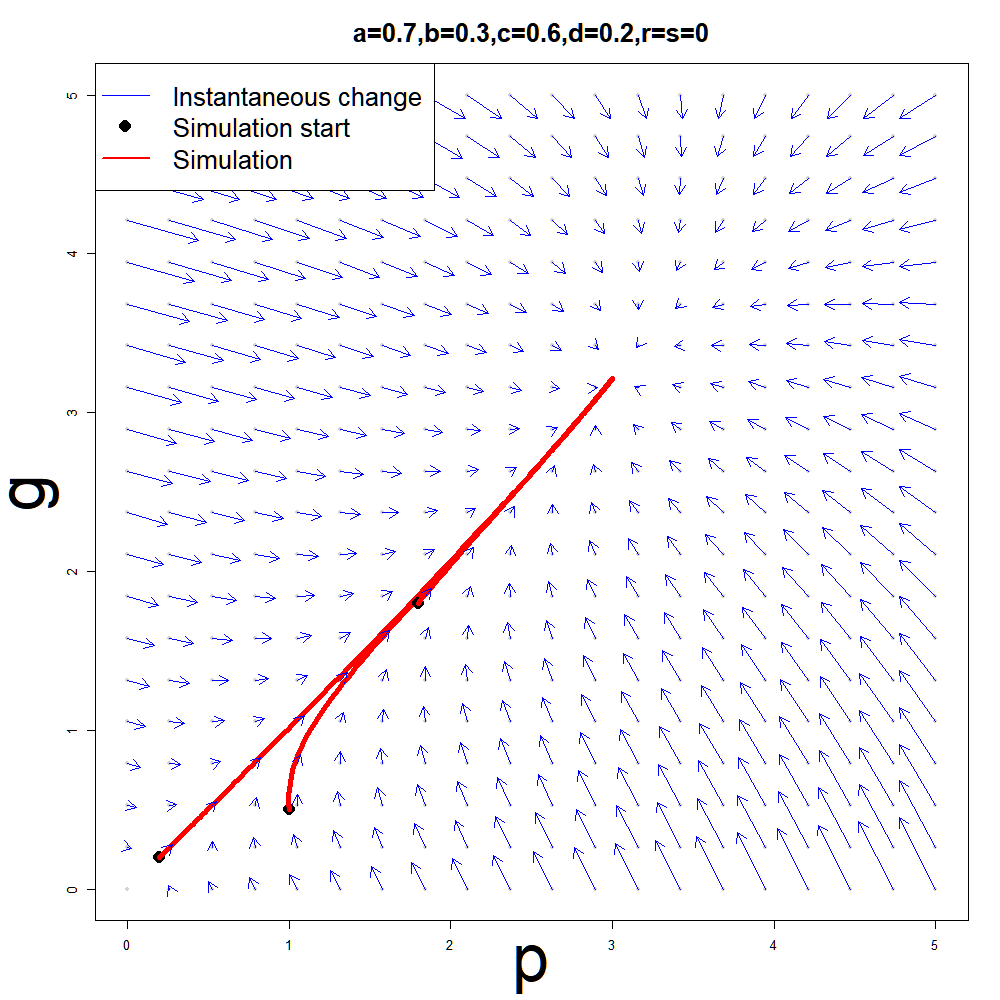
\includegraphics[width=\linewidth]{S2_one_equil.png}\\
%     \small Stabilized spending

%     \column{0.33\textwidth}
%     \centering
%     \textbf{$r,s=1$}\\
%     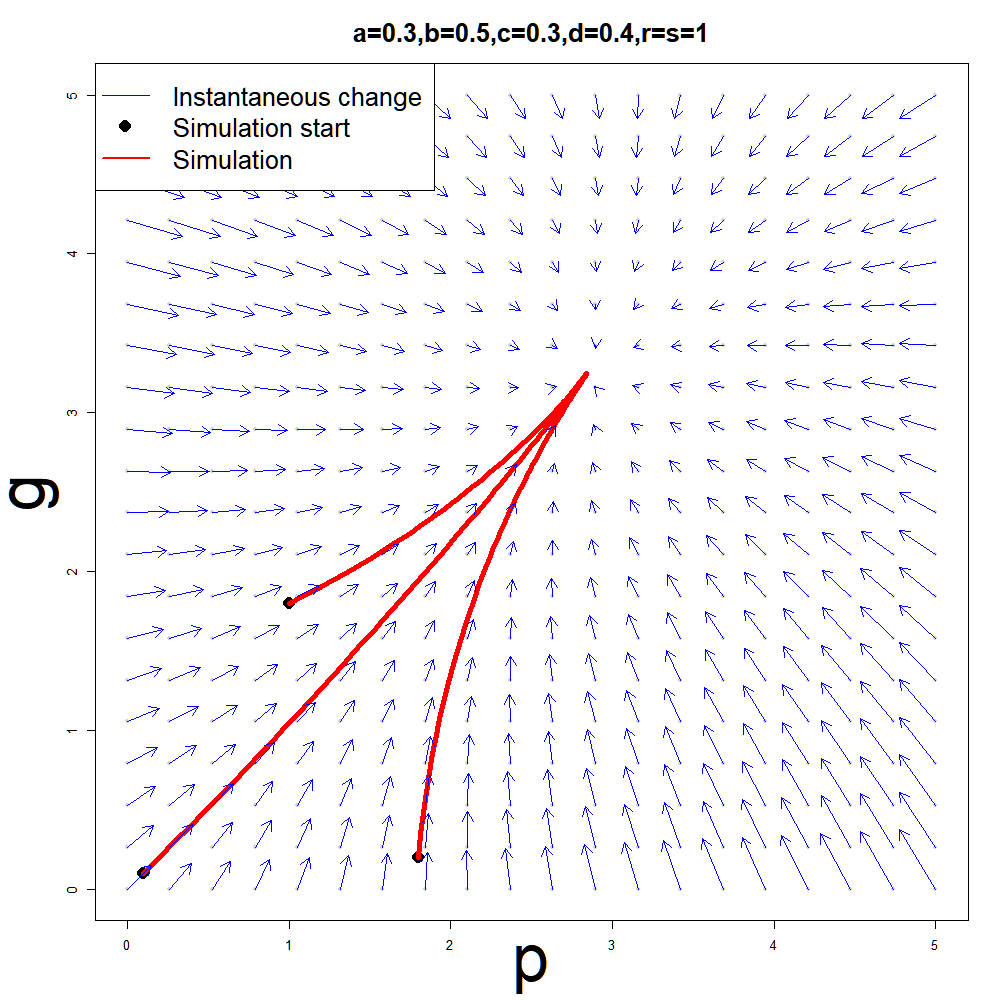
\includegraphics[width=\linewidth]{S3_grievance_unique.png}\\
%     \small Unique equilibrium based on trust/hostility
% \end{columns}

%\vspace{0.4cm}

% \begin{itemize}
%     \item Stability depends on relative strength of fear ($b,d$) vs restraint ($a,c$)
%     \item Convergence:
%     \begin{itemize}
%         \item $bd > ac$ $\rightarrow$ decay to zero (disarmament)
%         \item $bd = ac$ $\rightarrow$ steady-state equilibrium
%         \item $bd < ac$ $\rightarrow$ unbounded growth (arms race)
%     \end{itemize}
% \end{itemize}

%\end{frame}

% \section{End}
\section{Conclusion and Next Steps}

\begin{frame}{Conclusion and Next Steps}

\vspace{0.1cm}

    
        \begin{block}{Conclusion}
        \begin{itemize}
            \item \textbf{Base Model:} 
                In this model, long-term outcomes depend only on combined fear versus combined spending preservation.
            \item \textbf{Public Sentiment:} 
                Initial spending influences this model's behavior and shifts the equilibrium which makes stable positive spending more likely.
            \item \textbf{Mutual Logistic Fear:} This model accounts for economic limitations and prevents unending arms race with infinite spending.
        \end{itemize}
        \end{block}
       
        % \vspace{0.1cm}

        \begin{block}{Next Steps}
        \begin{itemize}
            \item Sensitivity Analysis
            \item Analytical solutions for equilibrium and stability
        \end{itemize}
        \end{block}
\end{frame}

\section{End}
{\BackgroundShaded
\begin{frame}
    \LARGE \textcolor{white}{Thank you for listening!}
    \footnotetext{\textcolor{white}{Presentation theme by Ricardo B. Lourenco}}
\end{frame}
}
\end{document}
